% HistoWeave -- Bioinformatics Original Paper, format-free initial submission
% Official requirements checked 2026-07-27:
% https://academic.oup.com/bioinformatics/pages/author-guidelines
% Claim posture: narrowed evidence-governance + selective abstention paper
% (not a validated personalised method-selector paper).
\documentclass[12pt]{article}

\usepackage[utf8]{inputenc}
\usepackage[T1]{fontenc}
\usepackage{amsmath,amssymb}
\usepackage{booktabs}
\usepackage{graphicx}
\usepackage{geometry}
\usepackage{hyperref}
\usepackage{lineno}
\usepackage{natbib}
\usepackage{setspace}
\usepackage{xcolor}

\geometry{margin=1in}
\graphicspath{{figures/}}
\hypersetup{colorlinks=true,linkcolor=blue,citecolor=blue,urlcolor=blue}
\doublespacing
\linenumbers

\newcommand{\software}{HistoWeave}
\newcommand{\required}[1]{\textcolor{red}{[AUTHOR REQUIRED: #1]}}

\title{\software: evidence-governed method decisions with structured abstention
for spatial transcriptomics}
\author{
\required{full author names and order}\\
\required{departments, institutions, cities, postal codes, and countries}\\
\required{corresponding author name, email, and ORCID}
}
\date{}

\begin{document}
\maketitle

\noindent\textbf{Article type:} Original Paper \hfill
\textbf{Subject category:} Gene expression

\begin{abstract}
\noindent\textbf{Motivation:} Spatial-domain methods are often compared across
incompatible tasks or with the true domain count supplied, yet decision tools
rarely refuse personalisation when evidence is insufficient.
\textbf{Results:} \software{} admits only task-compatible, source-verified
benchmark evidence and returns a method set, global default, evidence request,
or abstention. An 11-case audit admitted no incompatible evidence. Oracle
\(K\) cut SpaGCN ARI by more than half on one DLPFC section. Always-personalising
raised regret (0.047 versus 0.029). Registered HER2ST/CRC studies retained
global or evidence-required actions. On the aligned 13-unit non-oracle panel,
nested unit-holdout personalisation covered 5/13 units and lowered deployed
regret ($-0.0115$; 95\% CI $-0.0215$ to $-0.0029$); cross-study transport
remained fail-closed.
\textbf{Availability and Implementation:} BSD-3-Clause source, tests, and
frozen artefacts: \url{https://github.com/HERRY423/Histoweave};
\url{https://doi.org/10.5281/zenodo.21586217}.
\textbf{Contact:} \required{email}.
\textbf{Supplementary information:} Supplementary data are available online.
\end{abstract}

\section{Introduction}

Spatial transcriptomics couples molecular profiles to tissue coordinates and
has moved from array-based measurements to assays that resolve thousands to
millions of locations or cells \citep{stahl2016,maynard2021,chen2022,moses2022}.
The associated analysis ecosystem now contains spatially informed Bayesian,
graph-neural-network, and neighbourhood-augmentation methods, including
BayesSpace, SpaGCN, STAGATE, GraphST, and BANKSY
\citep{zhao2021,hu2021,dong2022,long2023,singhal2024}. These methods encode
different assumptions about whether neighbouring observations should share a
label, how expression and coordinates should be combined, and whether the
number of domains, \(K\), is known. Consequently, the best-performing method
can change with the assay, tissue, label semantics, and evaluation protocol
\citep{yuan2024}.

Benchmark tables do not by themselves define an actionable method decision.
Three recurrent problems are especially consequential. First, a clustering
method may receive the truth-derived \(K\) even though \(K\) is unknown in a
new experiment. Its adjusted Rand index (ARI) then measures performance under
oracle information rather than the intended deployment setting. Second,
``ground truth'' can denote contiguous anatomy, pathology regions,
transcriptomic cell types, or clusters produced by another algorithm. Pooling
these targets treats distinct questions as interchangeable. Third, a
data-dependent method selector can appear useful relative to random choice
while offering no advantage over the stronger rule of always choosing the
best method in the training data. Small within-study cross-validation further
obscures this distinction.

Existing spatial-omics frameworks solve complementary problems. SpatialData
provides a common data model, and Squidpy provides scalable spatial analysis
\citep{marconato2025,palla2022}. Large benchmarks map method behaviour across
technologies and organs and can list scenario-specific recommendations
\citep{yuan2024,chen2025imeta}, but a recommendation table is not itself an
executable, query-bound decision under incomplete evidence. Related
machine-learning work studies dataset-level algorithm selection under
distribution shift \citep{jiang2025ood} and selective prediction with
abstention and coverage constraints
\citep{geifman2017selective,casacuberta2025selective}; those results motivate
reporting risk conditional on action and refusing forced labels when evidence
is weak. What is missing in spatial transcriptomics practice is an executable
layer that decides which benchmark evidence is admissible for a declared task,
binds validation results to their source artefacts, and refuses to personalise
when those checks fail.

We developed \software{} as that decision layer. Its unit of output is not a
universal winner but a versioned \texttt{DecisionCard}: an auditable record of
admitted and rejected evidence, rule outcomes, selected method set,
comparators, required controls, and a claim boundary. Four actions are
possible: \texttt{personalised\_set}, \texttt{global\_default},
\texttt{evidence\_required}, and \texttt{abstain}. We evaluate the protocol
to test whether it fails closed under invalid evidence, whether silent
oracle-\(K\) use changes SOTA interpretation, and whether real external
evidence currently justifies personalisation. The experiments do not establish
a new clustering algorithm or a validated cross-study meta-selector
(Table~\ref{tab:claims}).

\begin{table}[t]
\centering
\caption{\textbf{Scientific claim boundary for this Original Paper.}}
\label{tab:claims}
\begin{tabular}{@{}p{0.46\textwidth}p{0.46\textwidth}@{}}
\toprule
\textbf{We claim} & \textbf{We do not claim} \\
\midrule
Evidence semantics and source integrity can
be machine-checked before aggregation &
Nearest-neighbour ranking or Pareto sorting is a new algorithm \\
Cross-task, circular, proxy-domain, and
undeclared oracle-\(K\) evidence is rejected
rather than softly mixed &
Soft down-weighting makes incompatible
evidence valid \\
A decision may be a non-dominated set, a
global fallback, an evidence request, or
abstention &
A local ranking proves one method is
biologically correct \\
Negative or missing held-out evidence must
change the action &
Reference-neighbour fit is independent
generalisation proof \\
Oracle access to \(K\) can materially change
reported ARI and must be dual-tracked &
A universal penalty converts oracle-\(K\)
scores into non-oracle performance \\
On registered prospective studies without an
aligned development panel the protocol retains
global or evidence-required actions &
Cross-study transport personalisation is
validated between HER2ST and CRC \\
On an aligned 13-unit non-oracle multi-study
panel, nested unit-holdout gating can yield
nonzero coverage and lower deployed regret &
Personalised selection is universally superior
on every unseen study or assay \\
\bottomrule
\end{tabular}
\end{table}

\begin{figure}[t]
\centering
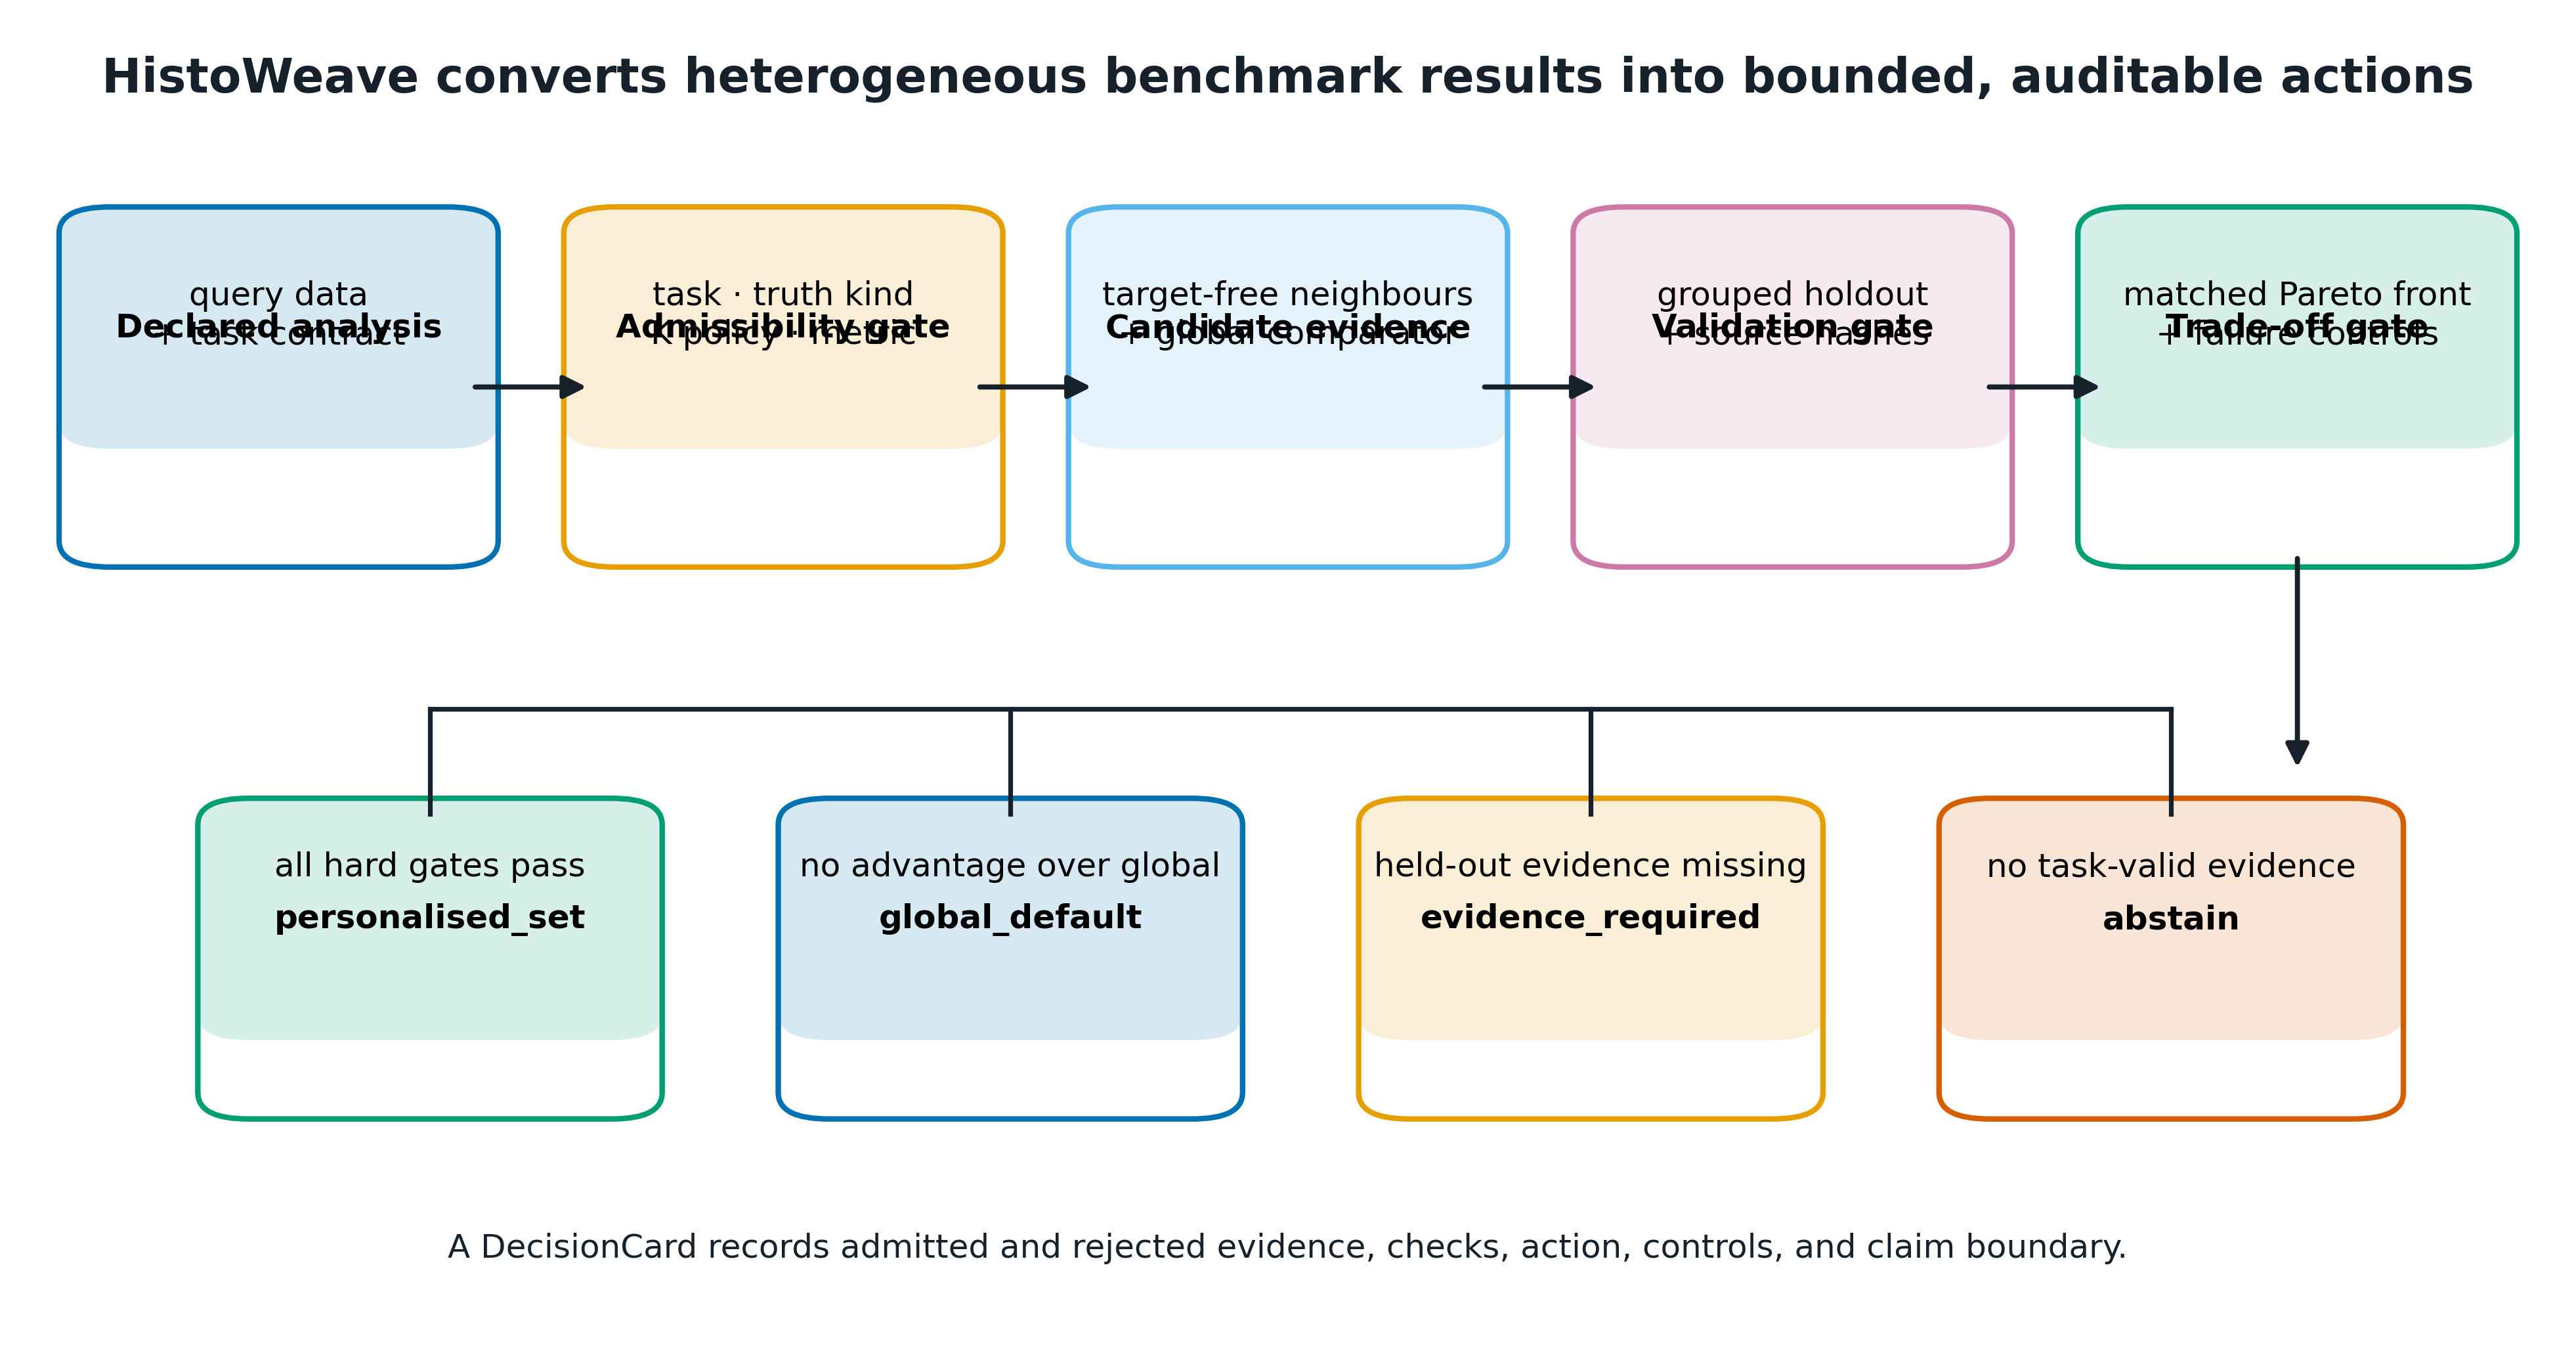
\includegraphics[width=\textwidth]{figure1_workflow.png}
\caption{\textbf{Evidence-governed decision workflow.} A declared task and
query enter sequential admissibility, candidate, validation, and trade-off
gates. The output is one of four actions. \texttt{Global\_default} means that
task-valid evidence exists but does not justify personalisation;
\texttt{abstain} is reserved for the absence of task-valid evidence. Every
check and rejected evidence object is recorded in a \texttt{DecisionCard}.}
\label{fig:workflow}
\end{figure}

\section{System and methods}

\subsection{Decision problem and output actions}

Let \(q\) be a query dataset, \(\tau\) its declared analysis task, and
\(\mathcal{E}\) a collection of benchmark evidence. A selector proposes a
ranked list \(R(q,\mathcal{E})\), but \software{} treats that list as a
reference-data proxy rather than as a decision. A policy
\(\pi(q,\tau,\mathcal{E})\) converts the proxy and its validation evidence
into an action \(a\) and a set of methods \(M\):
\[
  \pi(q,\tau,\mathcal{E}) \longrightarrow
  (a,M), \qquad
  a \in
  \{\texttt{personalised\_set},\texttt{global\_default},
  \texttt{evidence\_required},\texttt{abstain}\}.
\]
The action is \texttt{personalised\_set} only when every hard evidence
contract passes, the query-local proxy beats the training-fold global
comparator, suitable grouped held-out validation supports that advantage, and
any supplied matched Pareto table retains at least one proposed
configuration. Missing held-out validation yields
\texttt{evidence\_required}; lack of local advantage yields
\texttt{global\_default}; absence of task-valid evidence yields
\texttt{abstain} (Fig.~\ref{fig:workflow}).

The default policy requests a shortlist of at most three configurations,
support from at least two reference units, and a rank-support heuristic of at
least 0.25. The heuristic describes agreement among neighbours; it is not
reported as a calibrated probability. Policy thresholds are serialized in
the card so that changing a threshold creates a distinguishable policy.

\subsection{Evidence schema and fail-closed admissibility}

Each evidence object declares its task, ground-truth kind, \(K\) policy,
metric direction, method panel, split unit, training exclusion status, and
source artefacts. \software{} admits a reference only when its task and
ground-truth semantics are compatible with the query. Cluster-proxy,
self-supervised, Leiden, and Louvain labels cannot serve as ground truth for
spatial-domain recovery. Cross-modal domain partitions are isolated rather
than softly down-weighted. The default decision policy rejects undeclared or
oracle-\(K\) evidence for a non-oracle query.

Validation JSON is not trusted by filename alone. The loader verifies the
SHA-256 digest of every bound source artefact and retains the verified paths
in a typed object. The decision engine then checks the validation task,
ground-truth kind, \(K\) policy, metric, method panel, split unit, sample
count, and training exclusion statement against the recommendation contract.
An unverified dictionary, a mismatched panel, or a changed source file cannot
unlock \texttt{personalised\_set}.

\subsection{Candidate generation and global comparator}

Candidate generation uses target-free dataset descriptors stored in a
landscape knowledge base. Continuous descriptors are imputed and standardized
using reference-only statistics. Cosine similarity retrieves the \(k\)
nearest admissible references; task and platform matches can increase prior
weight only after hard admissibility has passed. A method configuration is
identified by both its base method and its spatial-context setting (for
example, \texttt{spectral@sw0.3}), preventing parameterizations with distinct
behaviour from being collapsed.

For each method, \software{} calculates a similarity-weighted reference score,
support, coverage, uncertainty, and rank-support heuristic. The global
comparator is selected using training references only. Selection regret on a
held-out unit \(i\) is
\[
  r_i = s_{i,m_i^\ast} - s_{i,\widehat m_i},
\]
where \(s_{i,m_i^\ast}\) is the best finite ARI in the fixed method panel and
\(s_{i,\widehat m_i}\) is the ARI of the selected method. A personalised
policy must be compared with the training-fold global method, not only with a
random-choice expectation. Deployed regret is also reported under the action
actually taken by a policy (global, ungated \(k\)-NN, or \software{}), which
can differ from the regret of a forced personalised shortlist.

\subsection{Pareto set and post-hoc spatial information}

When matched measurements are available, configurations are compared on ARI
(maximize), runtime (minimize), memory (minimize), and bootstrap ARI interval
width (minimize). A configuration is retained only if no other configuration
is at least as good on every observed objective and strictly better on at
least one. The decision set is the ordered intersection of the candidate
shortlist and this non-dominated frontier.

\software{} also implements an information-theoretic spatial utility score
(ISUS),
\[
  \mathrm{ISUS} = \frac{I(D;S\mid E)}{I(D;E)},
\]
where \(D\) denotes trusted domain labels, \(S\) coordinates, and \(E\)
expression features. Mutual information is estimated with a mixed
discrete--continuous \(k\)-nearest-neighbour estimator \citep{ross2014}.
Because ISUS requires trusted labels, it is a post-hoc descriptor and never a
pre-execution selection gate. Coordinate-shuffle nulls and a paired
ISUS--ARI-gain audit are retained to prevent the ratio from being interpreted
as an unvalidated predictor.

\subsection{Evaluation design and evidence tiers}

Because the scientific product is a decision protocol rather than a trained
classifier, experiments are organised by the claim they can support
(Table~\ref{tab:tiers}).

\begin{table}[t]
\centering
\caption{\textbf{Evidence tiers used in this paper.} Higher tiers do not
supersede lower-tier claim boundaries; each tier answers a different
question.}
\label{tab:tiers}
\begin{tabular}{@{}llp{0.42\textwidth}@{}}
\toprule
\textbf{Tier} & \textbf{Material} & \textbf{Question answered} \\
\midrule
T0 & 11 adversarial decision-card cases &
Does the implemented path fail closed for enumerated contract violations? \\
T1 & Five DLPFC sections, 20 configurations;
oracle-\(K\) versus estimated-\(K\) ablations &
How does access to true \(K\) change ranking and ARI interpretation? \\
T2 & Historical five-study oracle-\(K\) landscape &
How heterogeneous are descriptive method rankings across platforms?
(not a validation split) \\
T3 & 20 study-grouped selective queries &
Does personalisation improve regret--coverage over always-global? \\
T4 & Two registered prospective external studies: HER2ST donors and CRC
patients (non-oracle \(K\)) &
Without an aligned development panel, does evidence justify personalisation
on untouched studies? \\
T4b & Aligned HER2ST+CRC non-oracle meta-panel (13 strict units); nested
unit-holdout gated 1-NN &
On the completed multi-study panel, can personalisation improve deployed
regret with nonzero coverage? (not cross-study transport) \\
T5 & Fixed development/calibration/test synthetic construct panel &
Can the selector improve choices under a true switch while remaining safe
under an independent no-signal condition? \\
\bottomrule
\end{tabular}
\end{table}

\paragraph{Development and sensitivity (T1).}
The DLPFC development track used five sections from the LIBD study
\citep{maynard2021}. It contains 20 configurations: five general clustering
algorithms at three spatial weights and five spatially informed methods.
Oracle-\(K\) runs support bounded benchmarking and sensitivity analysis only.
Silhouette, spatial-silhouette, and ensemble estimates of \(K\) provide the
non-oracle track for SpaGCN and STAGATE at seed 42.

\paragraph{Historical descriptive landscape (T2).}
A separate external panel contains five datasets from independent studies
spanning Visium HD, Xenium, Xenium Prime, Visium, and MERFISH. Fifteen methods
were prespecified; 13 produced finite results on all five datasets. Only
BANKSY overlaps the five spatially informed DLPFC families, so the two panels
are never pooled as an aligned state-of-the-art comparison. This historical
oracle-\(K\) landscape is descriptive only: it is not a cross-validation
estimate, does not train or validate the selector, and contributes no evidence
to the personalised-selection claim.

\paragraph{Selective regret--coverage (T3).}
A frozen selective endpoint comprises 20 study-grouped queries. For each
confidence threshold we record personalisation coverage and mean deployed
regret of always-personalised, always-global, and selective policies.

\paragraph{Primary external validation (T4).}
The primary external validation uses HER2ST legacy Spatial Transcriptomics
breast-cancer donors with pathologist region labels
\citep{andersson2021}. Public registration of the protocol, exclusion rules,
method panel, non-oracle \(K\) estimator, seeds, and success criteria preceded
access to outcome-bearing files (GitHub issue~19; server timestamp
2026-07-29T05:34:31Z; protocol commit and SHA-256 recorded in the repository
freeze). Predictions and comparator actions were frozen before a separate
scorer opened labels. The analysis unit is the donor. Seven donors were
evaluable after the locked exclusion of G2 for duplicated label coordinates.
Nine methods (SpaGCN, STAGATE, GraphST, BayesSpace, BANKSY, spectral,
Gaussian mixture, \(k\)-means, agglomerative) shared the same retained spots,
raw-count start, seed grid, and label-free estimated \(K\). Backend failures
were retained without silent substitution. Registration-time development
evidence selected SpaGCN as the global default. An ungated 3-NN rule was
frozen as an existing-rule comparator.

A second public registration (GitHub issue~20) locked 14 CRC Visium sections
from seven patients, the same nine methods, three seeds, patient-level
aggregation, and one shared non-oracle \(K\) per section before data access.
All policy actions were frozen as \texttt{evidence\_required} because the
registered development meta-panel minimum was not met. Predictions and
failures were frozen before the official pathologist annotations were
downloaded. The strict descriptive endpoint uses one seven-patient complete
mask across all nine methods. Fifteen A120838 deep-method attempts were stopped
for repeated infrastructure/runtime limits after outcome sealing and retained
as failures without imputation; the patient remained evaluable from Rep1 seed
42, as permitted by the registered replicate-failure rule.

\paragraph{Construct validity (T5).}
A fixed-split synthetic experiment separates development fitting, threshold
calibration, and two independent test panels. A target-free feature truly
switches the better method in the signal panel; the null panel contains no
local switch and keeps the training-derived global method optimal. A ridge
method-score model and predicted-gain gate are fitted without test outcomes.
This tests improved choices and no-signal safety, not biological validity.

\paragraph{Secondary oracle stress test.}
A six-section breast-cancer Visium cohort from Wu \textit{et al.}
\citep{wu2021} remains a secondary, oracle-\(K\), one-shot stress test fixed
before local outcome execution but without an independent public timestamp. It
is reported only as supporting negative stress evidence and does not satisfy
the non-oracle external gate.

\subsection{Benchmarks and statistical analysis}

ARI \citep{hubert1985} is the primary accuracy metric. DLPFC configurations
were run with seeds 42, 1, and 2 using truth-derived \(K\) unless stated.
External panel scores are means over the same three seeds. For HER2ST, mean
deployed regret and percentile bootstrap 95\% confidence intervals resample
donors. The locked decision uses the prespecified point-estimate margin; the
interval is descriptive because all units arise from one study. Non-inferiority
to always-global is reported only when actions differ; action identity yields
zero regret difference by definition and is not interpreted as selection
advantage.
For CRC, ARI is calculated per section and seed, successful seeds are averaged
within section, and sections are averaged within patient. Same-mask summaries
remain stratified by study; no pooled donor/patient bootstrap treats studies as
exchangeable. Runtime skips and backend failures remain in the failure ledger.

The adversarial audit exercises the complete decision-card path. Nine invalid
cases independently introduce cross-task evidence, cluster-proxy truth,
missing \(K\) policy, oracle \(K\), missing metric declaration, unverified
validation, or mismatched validation task, panel, or \(K\) policy. Two valid
controls include one ordinary admissible case and one case in which the
locally ranked candidate is Pareto-dominated. We report incompatible-evidence
admission, valid-evidence false rejection, and dominated-selection rates.

\subsection{Implementation and reproducibility}

\software{} is implemented in Python 3.11 or later and distributed as
\texttt{histoweave-spatial} under the BSD-3-Clause license. The core depends
on AnnData, NumPy, pandas, scikit-learn, SciPy, and SpatialData
\citep{pedregosa2011,marconato2025}. The \texttt{SpatialTable} abstraction
records structured provenance. Plugins declare task categories, optional
dependencies, and maturity tiers. Containerized adapters for STAGATE,
GraphST, and BayesSpace fail closed if their external environments are
unavailable; they do not substitute an easier fallback while retaining the
original method name.

The submission freeze contains source hashes, generated artefact hashes,
method-coverage ledgers, and a reproduction checker. Figure source code reads
only frozen CSV/JSON artefacts. Raw public datasets are not redistributed;
preparation scripts and persistent dataset identifiers document acquisition
and transformation.

\section{Results}

Results follow the claim tiers in Table~\ref{tab:tiers}. Positive language is
reserved for contracts that fire correctly and for measurement findings
(oracle-\(K\) sensitivity). Decision-policy results are reported as action
outcomes; they are not reframed as selector superiority.

\subsection{Fail-closed contracts reject incompatible evidence}

All 11 adversarial cases produced their prespecified outcome. None of the nine
invalid evidence objects unlocked personalisation, neither valid control was
falsely rejected, and the dominated candidate was not selected. The resulting
incompatible-admission, false-rejection, and dominated-selection rates were
all 0/eligible cases. These are software-contract tests rather than estimates
of error rates in an open population, but they demonstrate that the
implemented path fails closed for each enumerated incompatibility.

\subsection{Oracle access to \(K\) changes SOTA magnitude and interpretation}

Across the five DLPFC sections and three seeds, STAGATE had the highest grand
mean ARI (0.353), followed by BayesSpace (0.326) and SpaGCN (0.317)
(Fig.~\ref{fig:dlpfc}A). No method led every section. Section 151669 was
difficult for all configurations (maximum mean ARI 0.249), whereas on section
151670 \texttt{spectral@sw0.3} reached 0.346 and exceeded every spatially
informed method in this panel.

Providing \(K\) changed both the magnitude and interpretation of performance
(Fig.~\ref{fig:dlpfc}B). For SpaGCN, mean ARI decreased from 0.299 with
truth-derived \(K\) to 0.237 with silhouette-estimated \(K\). The largest
decline occurred on section 151673, from 0.418 at \(K=7\) to 0.186 at
estimated \(K=2\), a 55.5\% relative decrease. STAGATE decreased from 0.232 to
0.219 on average. None of the blind estimators recovered the true \(K\) on any
of the five sections. The effect was not monotone: on section 151670, \(K=2\)
produced higher ARI than truth-derived \(K=5\). These results support dual-track
reporting of oracle and estimated \(K\); they do not supply a universal
correction factor for published oracle-\(K\) tables.

\begin{figure}[t]
\centering
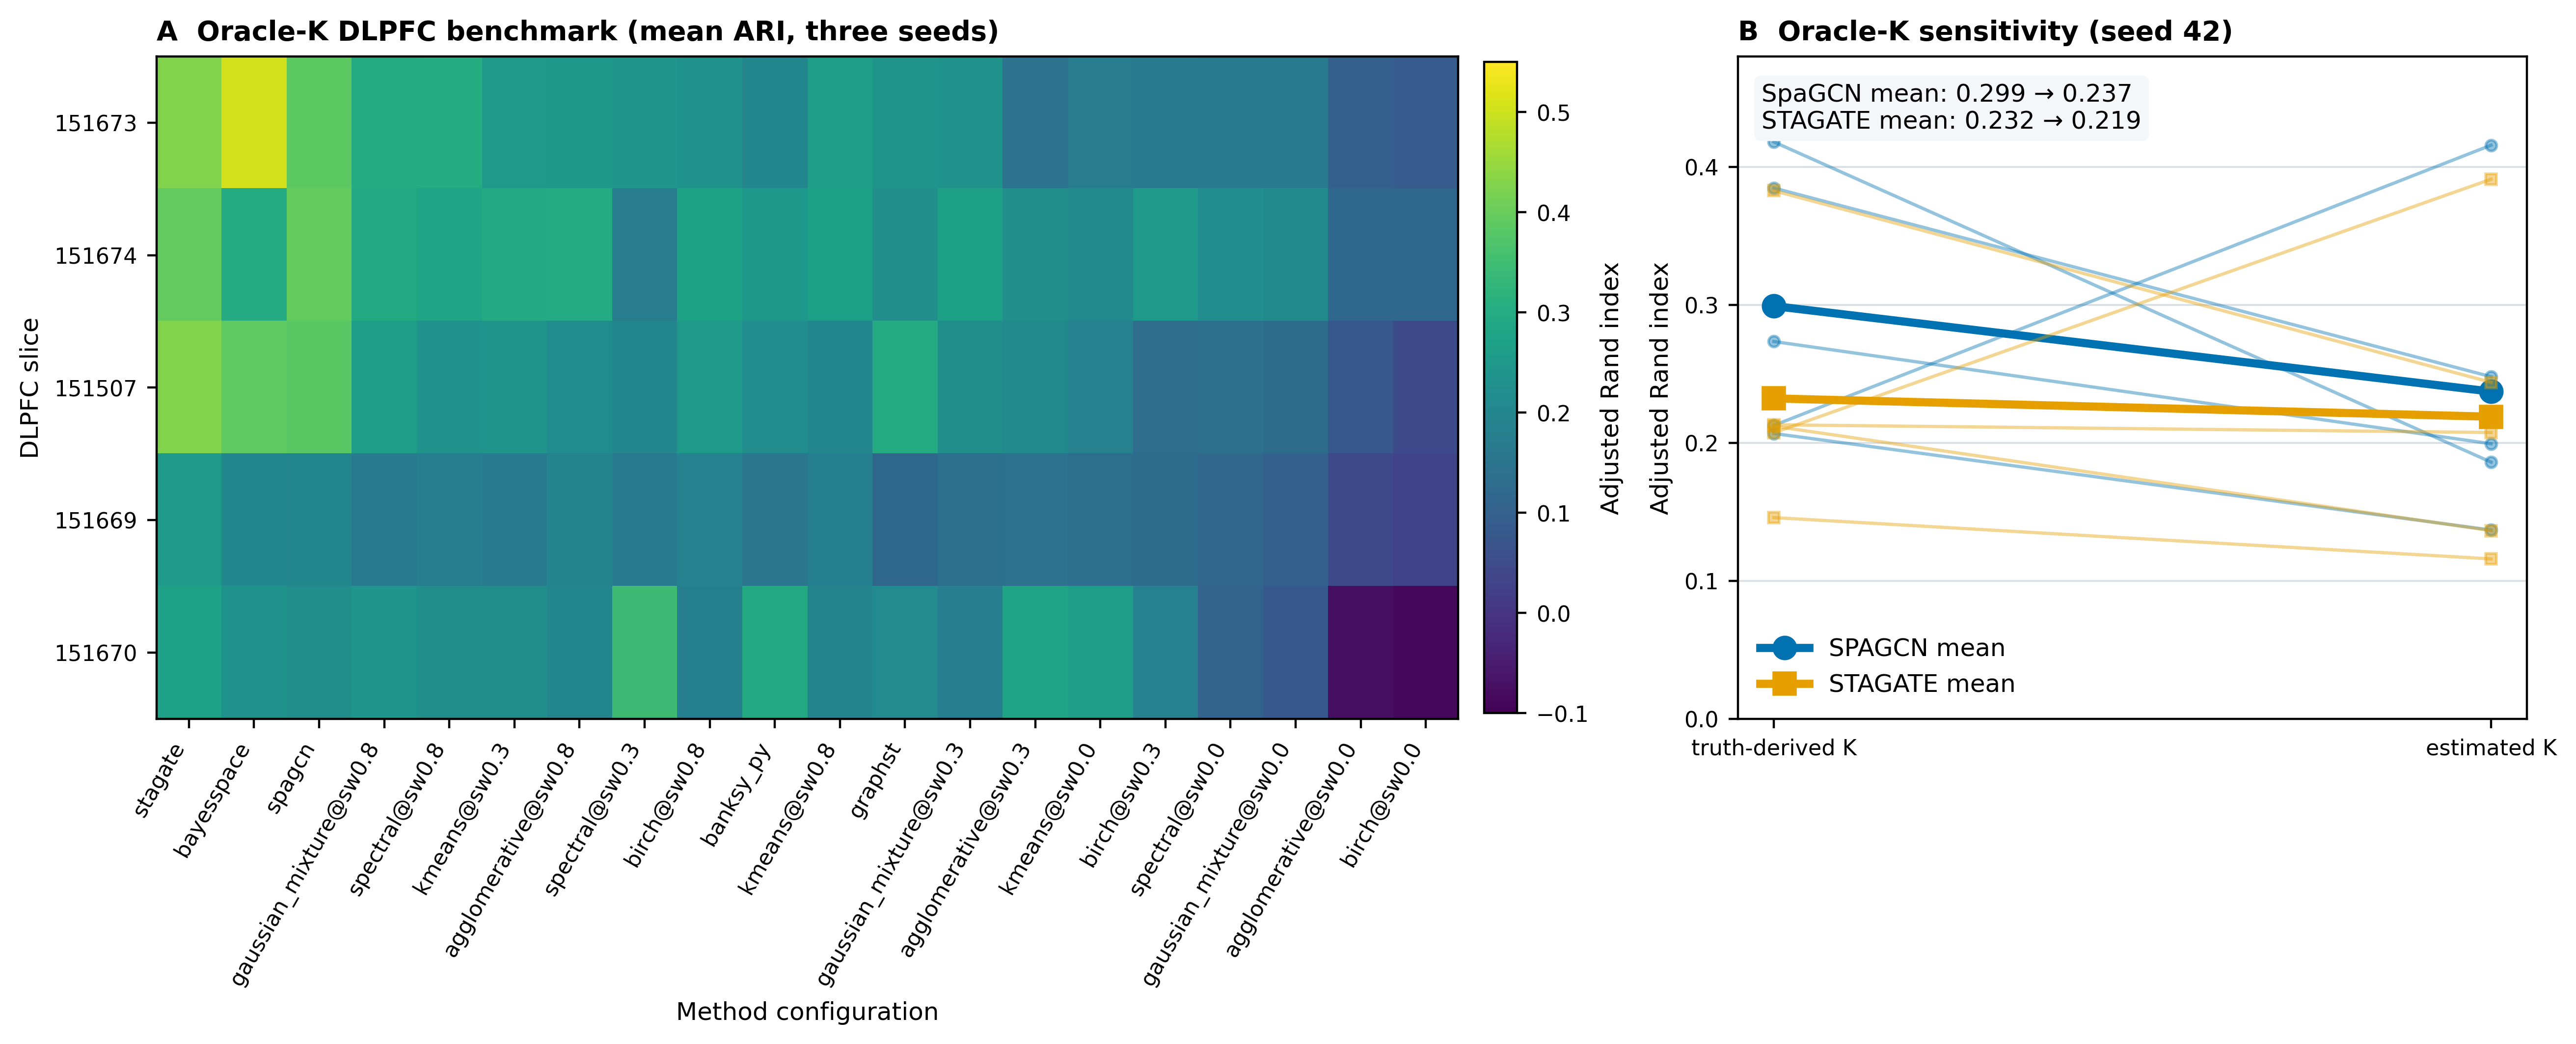
\includegraphics[width=\textwidth]{figure2_dlpfc_oracle_k.png}
\caption{\textbf{DLPFC benchmark and oracle-\(K\) sensitivity.}
\textbf{(A)} Mean ARI for 20 method configurations on five DLPFC sections
(three seeds, truth-derived \(K\)); columns are ordered by grand mean.
\textbf{(B)} Section-level ARI for SpaGCN and STAGATE using truth-derived or
silhouette-estimated \(K\) at seed 42. Thin lines denote sections and thick
lines denote method means.}
\label{fig:dlpfc}
\end{figure}

\subsection{Historical external landscape is descriptive only}

The five external datasets differed strongly in absolute difficulty and
method ranking (Fig.~\ref{fig:external}). Spectral clustering led four
datasets, with mean ARI ranging from 0.282 on MERFISH mouse brain to 0.676 on
Visium HD colorectal cancer. Mean shift led the Xenium lung dataset at 0.183.
The panel is incomplete for aligned SOTA comparison and uses oracle \(K\).
Consequently it is reported only to show rank heterogeneity across platforms;
no cross-validation accuracy, regret, or candidate-generator comparison from
these five units is used as validation evidence.

\begin{figure}[t]
\centering
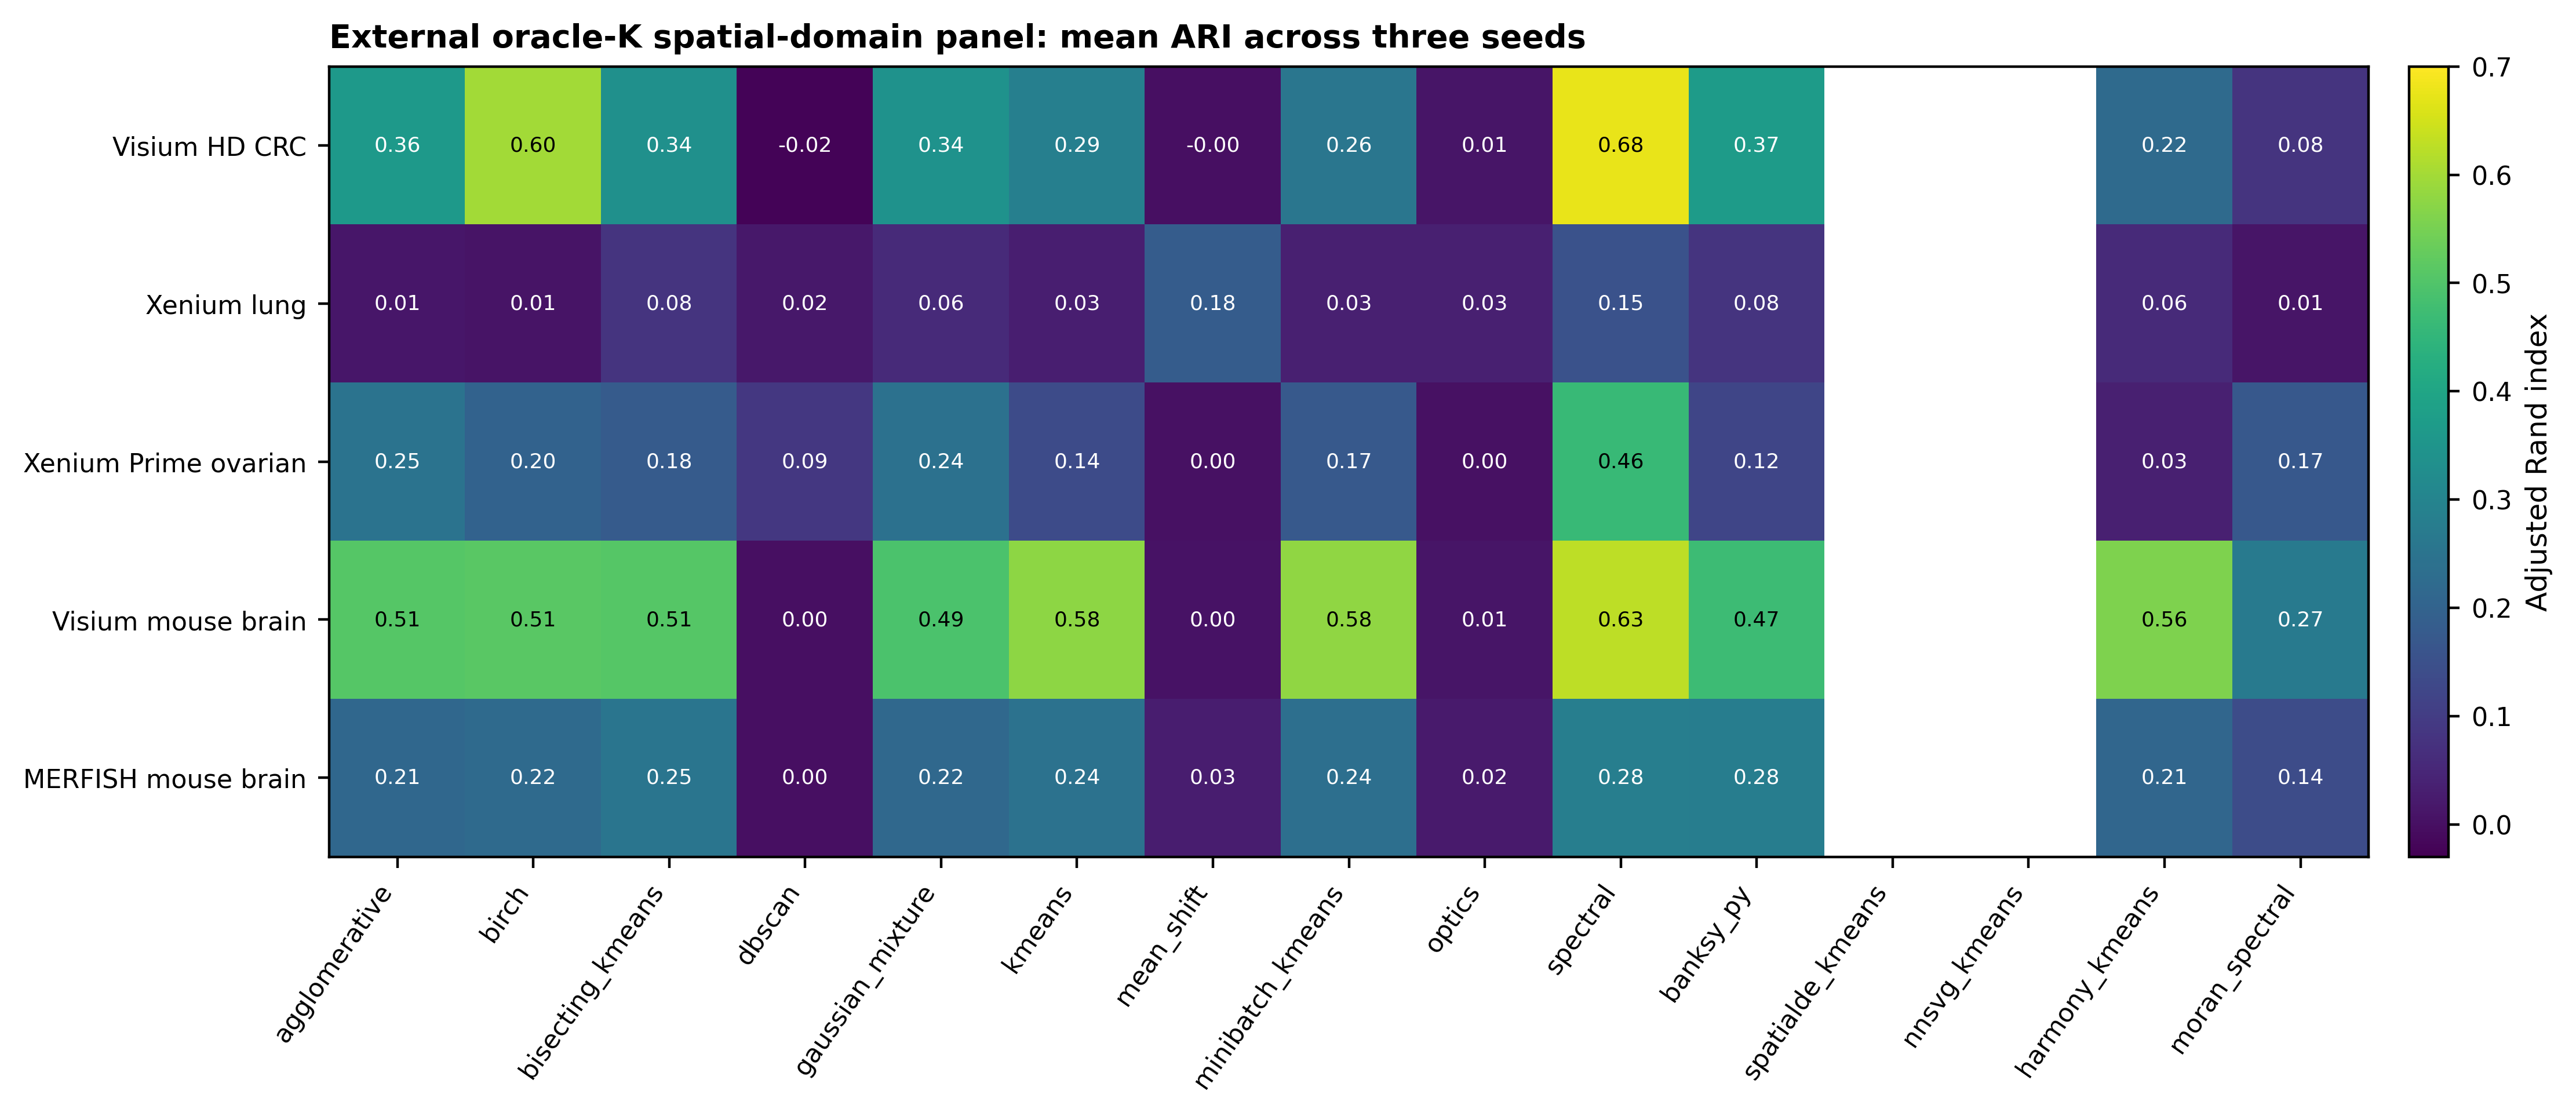
\includegraphics[width=\textwidth]{figure3_external_panel.png}
\caption{\textbf{External oracle-\(K\) spatial-domain panel (diagnostic).}
Cells show mean ARI over three seeds. The panel prespecified 15 methods; two
methods without finite results are blank. These datasets use anatomical,
pathology, or manual spatial-region labels. SpaGCN, STAGATE, GraphST, and
BayesSpace were not run across this panel, so the figure is not an aligned
comparison of the five DLPFC spatial-method families.}
\label{fig:external}
\end{figure}

\subsection{Selective evaluation retains the global default}

Across 20 grouped queries, always-personalised selection had mean regret
0.0468, whereas the training-fold global policy had mean regret 0.0290. The
selective action attained its minimum only at zero personalisation coverage
(Fig.~\ref{fig:validation}A). \software{} therefore returned the global
default throughout the observed confidence-threshold grid. This is a negative
decision result: the protocol prevented a higher-regret action rather than
demonstrating that the ranking heuristic was successful.

\subsection{Prospective non-oracle external validation yields zero personalisation
coverage}

On HER2ST, every method used the same non-oracle estimated \(K\), spots, and
seeds. On the strict nine-method six-donor mask, mean donor ARI ranged from
0.220 (BANKSY) to 0.131 (BayesSpace); SpaGCN, the locked global default from
registration-time development evidence, averaged 0.151
(Table~\ref{tab:her2st}). Seven available donors cannot establish a universal
ranking; the table is descriptive context for the decision comparison only.

\begin{table}[t]
\centering
\caption{\textbf{HER2ST aligned non-oracle panel (descriptive).} Strict
nine-method six-donor mask; estimated \(K\); three seeds.}
\label{tab:her2st}
\begin{tabular}{@{}lrr@{}}
\toprule
Method & Donors & Mean donor ARI \\
\midrule
BANKSY & 6 & 0.220 \\
STAGATE & 6 & 0.186 \\
GraphST & 6 & 0.182 \\
Agglomerative & 6 & 0.154 \\
Gaussian mixture & 6 & 0.152 \\
SpaGCN (locked global default) & 6 & 0.151 \\
\(k\)-means & 6 & 0.150 \\
Spectral & 6 & 0.146 \\
BayesSpace & 6 & 0.131 \\
\bottomrule
\end{tabular}
\end{table}

Because grouped, aligned full-panel development validation was unavailable at
registration, \software{} selected the pre-registered SpaGCN global default for
all seven donors. Personalisation coverage was 0/7 at every locked threshold,
including 0.25. The ungated 3-NN comparator selected
\texttt{gaussian\_mixture@sw0.8} on every donor with finite Gaussian-mixture
results. On the six-donor common-availability mask, \software{} minus
always-global deployed regret was 0.0000 by action identity (always-global
deployed regret 0.125, 95\% donor bootstrap CI 0.065--0.183). \software{} minus
ungated 3-NN deployed regret was 0.0002 (95\% CI \(-0.089\) to \(0.092\)).
Passing a 0.02 non-inferiority margin under action identity is not evidence of
better selection. The result validates fail-closed behaviour on a publicly
time-stamped external study: the protocol refused personalisation because the
evidence needed to justify it was absent.

The second outcome-sealed CRC study completed the nine-method common mask for
all seven patients (Table~\ref{tab:crc}). Mean patient ARI ranged from 0.145
(BayesSpace) to 0.200 (\(k\)-means); SpaGCN averaged 0.192. Patient-level
winners were heterogeneous: \(k\)-means led two patients, SpaGCN two, and
STAGATE, BANKSY, and Gaussian mixture one each. This differs from HER2ST, where
BANKSY led the strict six-donor common mask (0.220). Thus the two studies supply
13 independent same-mask units and a genuine cross-study rank reversal, not a
universal winner. All seven CRC actions were already frozen as
\texttt{evidence\_required}; the descriptive winner table cannot be converted
post hoc into a personalised-policy success.

\begin{table}[t]
\centering
\caption{\textbf{CRC aligned non-oracle panel (descriptive).} Seven-patient
same mask; sections and seeds are nested technical units.}
\label{tab:crc}
\begin{tabular}{@{}lrr@{}}
\toprule
Method & Patients & Mean patient ARI \\
\midrule
\(k\)-means & 7 & 0.200 \\
SpaGCN & 7 & 0.192 \\
Agglomerative & 7 & 0.188 \\
GraphST & 7 & 0.183 \\
BANKSY & 7 & 0.175 \\
Gaussian mixture & 7 & 0.173 \\
Spectral & 7 & 0.172 \\
STAGATE & 7 & 0.172 \\
BayesSpace & 7 & 0.145 \\
\bottomrule
\end{tabular}
\end{table}

A secondary oracle-\(K\) Wu stress test failed its locked 0.02-ARI margin
(mean regret 0.131, 95\% bootstrap CI 0.034--0.236) and is consistent with not
promoting an unverified personalised policy, but it is not a non-oracle
prospective confirmation and is not shown in Fig.~\ref{fig:validation}.

\begin{figure}[t]
\centering
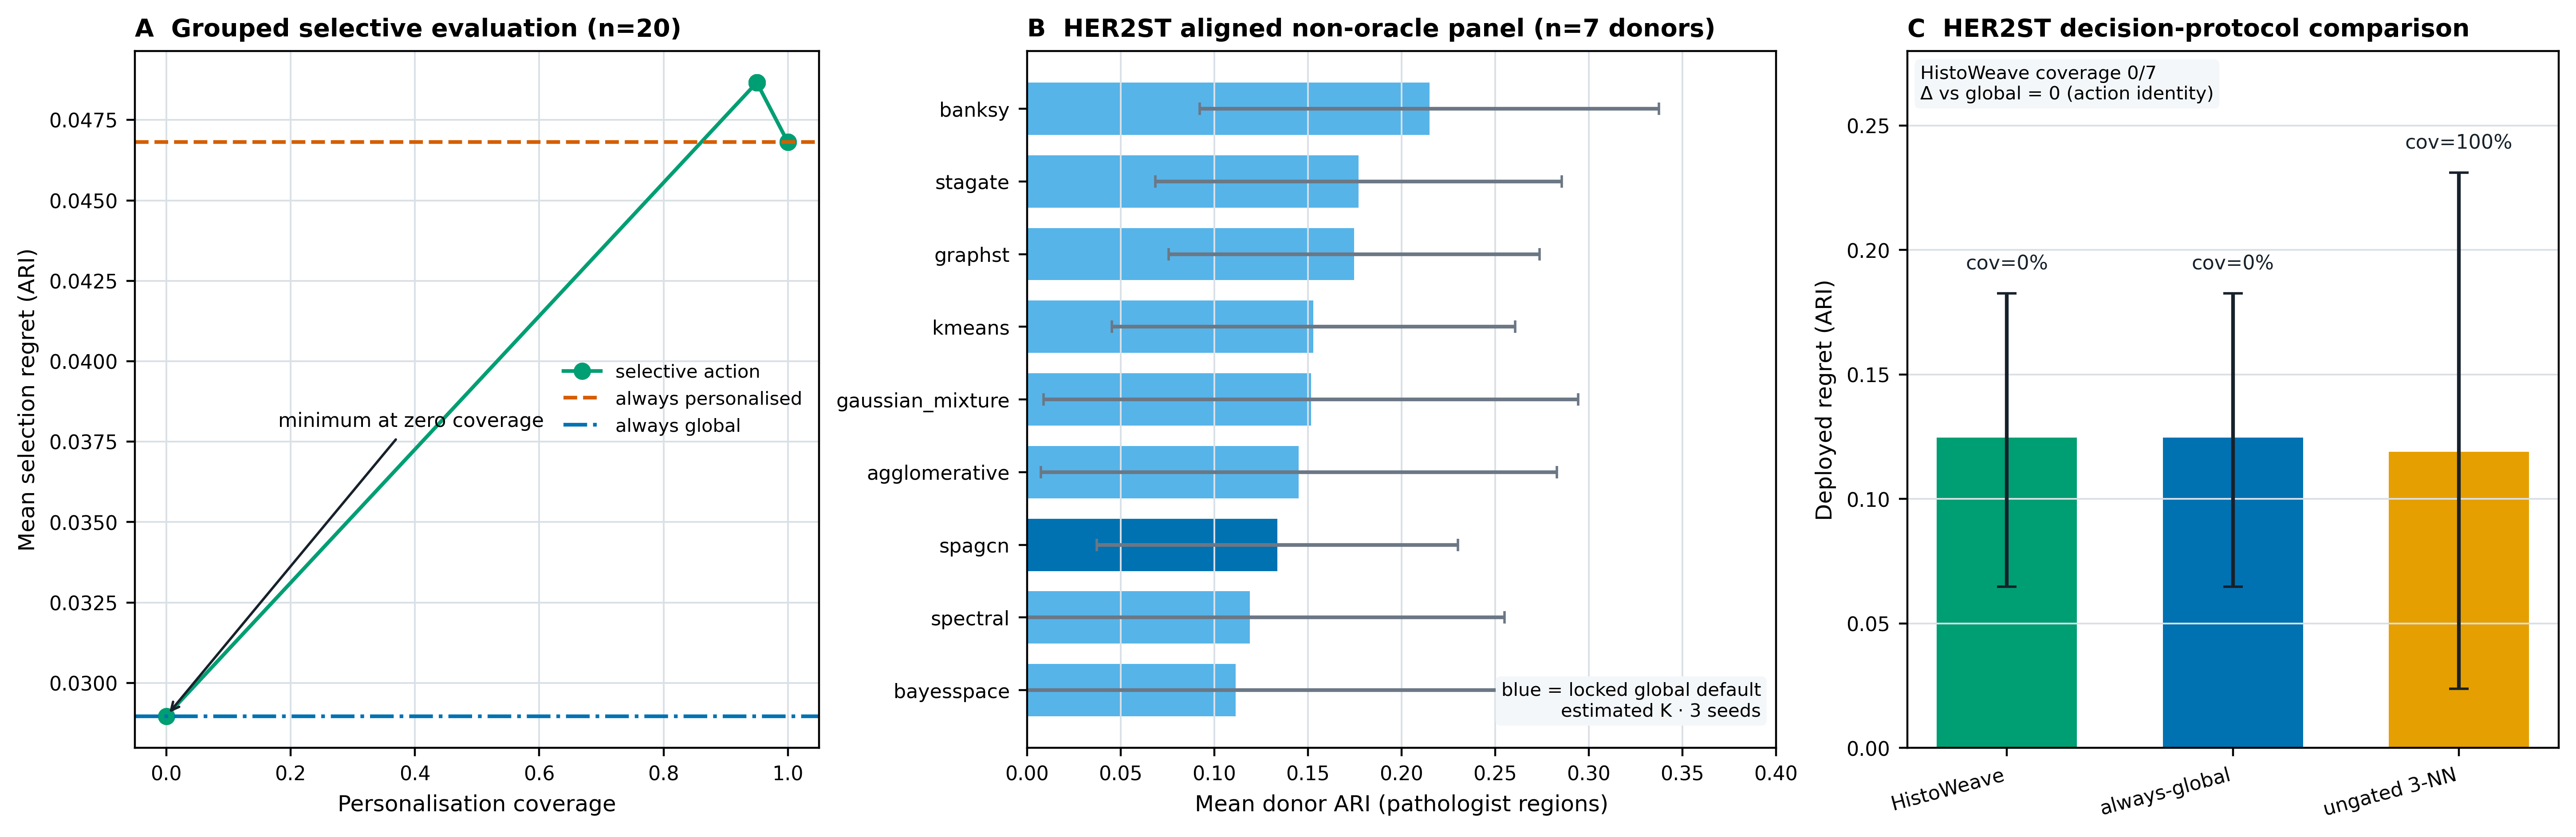
\includegraphics[width=\textwidth]{figure4_validation.png}
\caption{\textbf{Selective and HER2ST external validation preserve the
fallback.}
\textbf{(A)} Selective regret--coverage over 20 grouped queries; the minimum
is at zero personalisation coverage.
\textbf{(B)} HER2ST aligned non-oracle panel: mean donor ARI versus
pathologist regions (bars) with donor-level SD (whiskers); blue marks the
locked SpaGCN global default.
\textbf{(C)} HER2ST decision-protocol comparison of deployed regret
(donor-bootstrap 95\% CI). HistoWeave coverage is 0/7 and matches
always-global by action identity; ungated 3-NN covers available donors but
does not improve regret detectably. A secondary oracle-\(K\) Wu stress test
is reported in the text only.}
\label{fig:validation}
\end{figure}

\subsection{Aligned multi-study panel: nested unit-holdout personalisation improves
deployed regret}

After the two registered studies completed the same nine-method non-oracle
contract, their strict same-mask units formed an aligned development
meta-panel (six HER2ST donors and seven CRC patients; every method available
on all 13 units). Cross-study folds that trained on one study and tested on
the other remained fail-closed: calibration never unlocked
\texttt{personalised\_set}, so transport between HER2ST and CRC is
\textbf{not} claimed.

On the same 13-unit panel we evaluated a gated one-nearest-neighbour method
transfer under nested unit holdout: each donor or patient was held out once;
the gain threshold was chosen only on the remaining units using a
safety-first rule (coverage at least 0.2 and mean regret difference at most
zero; then lowest mean regret difference). Label-free features were restricted
to a small-n subset (library-size CV, spatial autocorrelation, effective rank,
and singular-value entropy). Nested unit-holdout coverage was 5/13 (0.385).
Mean deployed regret was 0.043 versus 0.054 for the training-fold global
method (BANKSY), a difference of \(-0.0115\) (donor/patient bootstrap 95\% CI
\(-0.0215\) to \(-0.0029\)). Covered units selected SpaGCN or \(k\)-means
rather than BANKSY. This is real-biology personalisation on independent units
from the aligned panel; it does not convert the earlier prospective
HER2ST/CRC freezes into personalised superiority, and it does not establish
cross-study transport.

A sequential confirmation protocol freezes this gated policy against a
HER2ST+CRC neighbour bank only and targets three LIBD DLPFC donors under the
same non-oracle nine-method contract. Public lock (commit and GitHub issue)
must precede DLPFC outcome scoring; DLPFC layer labels were previously used
for dual-track oracle-\(K\) reporting and are disclosed as such.

\subsection{Construct validity: fixed-split selection improves under a reliable signal}

The repaired T5 protocol retained the original malformed-predicate failure and
an intermediate null-safety failure, changed all generator/bootstrap seeds,
and evaluated a fixed ridge selector on new test units. The calibration rule
selected a predicted-gain threshold of 0.05 without test outcomes. On 120
signal-test units, coverage was 54/120 (0.45), every covered action chose the
planted best method, and recall among non-global opportunities was 0.857.
Deployed regret improved relative to always-global by \(-0.133\) (95\% paired
bootstrap CI \(-0.160\) to \(-0.107\)). On 120 independent no-signal units,
coverage and regret difference were both zero. Thus the corrected
implementation can improve selection under an identifiable switch and fail
closed without it. T5 remains construct validity only and does not replace the
aligned-panel nested unit-holdout result.

\subsection{Action frequencies and threshold sensitivity}

To test whether the four actions are only design diagrams, we re-applied the
default \texttt{DecisionPolicy} to the twenty study-grouped recommendation
objects without attaching a bound held-out validation pack
(Supplementary action-frequency and threshold tables). Under default settings
(\texttt{min\_rank\_support\_score}$=0.25$, \texttt{min\_support}$=2$,
\texttt{require\_heldout\_validation}$=$\texttt{true}), the protocol emitted
\texttt{evidence\_required} on 13/20 queries and \texttt{global\_default} on
7/20; \texttt{personalised\_set} and \texttt{abstain} were never selected.
The 13 \texttt{evidence\_required} outcomes are exactly the queries whose
local proxy beat the global comparator: missing grouped validation blocks
personalisation rather than silently promoting the shortlist. An ablation that
disables the held-out gate yields 12 \texttt{personalised\_set}, 7
\texttt{global\_default}, and 1 \texttt{evidence\_required}, confirming that
the gate---not rank-support alone---is the binding constraint on this cohort.

Sweeping \texttt{min\_rank\_support\_score}$\in\{0,0.15,0.25,0.40,0.50,0.75,0.90\}$
and \texttt{min\_support}$\in\{1,2,3\}$ with the held-out gate enabled never
unlocked \texttt{personalised\_set} (Supplementary threshold grid).
Thresholds therefore matter for local heuristics, but they cannot compensate
for missing validation evidence. On HER2ST, coverage remained 0/7 at every
locked threshold, so external risk--coverage is degenerate: the study
validates refusal (no unsupported personalisation), not a safer positive-coverage
operating point \citep{geifman2017selective}.

\section{Discussion}

\software{} addresses a different question from a new clustering algorithm or
from a comprehensive method ranking. Large spatial-clustering benchmarks such
as Chen \textit{et al.}\ \citep{chen2025imeta} are complementary: they
characterise method preferences across technologies, organs, and replicates and
can publish scenario tables. Our contribution is orthogonal---an executable
admissibility and selective-decision layer that refuses to treat those tables
as automatic deployment rules when task, \(K\) policy, panel alignment, or
grouped holdout contracts fail. Dataset-level algorithm selection under shift
\citep{jiang2025ood} and selective prediction with abstention
\citep{geifman2017selective,casacuberta2025selective} supply the right
evaluation language (risk conditional on coverage; forced prediction is not
always safer), which we instantiate for spatial-domain method choice with
source-hash-bound evidence.

The experiments illustrate why these constraints matter. On DLPFC, access to
truth-derived \(K\) changed SpaGCN ARI by more than half in one section, yet
the direction was not consistent across all sections. An oracle-\(K\) score
therefore cannot be translated into deployment performance by applying a
single penalty. On the diagnostic external panel, a high top-1 rate concealed
identical mean regret to the global method. Grouped selective analysis and the
HER2ST prospective study both retained the global default: the former because
always-personalising increased regret, the latter because the development
evidence required for personalisation was simply unavailable. Reporting these
outcomes narrows the claim to what the evidence supports---an auditable
fail-closed decision protocol---not a validated personalised selector.

Risk--coverage on the registered prospective studies is \emph{degenerate at
zero coverage} when the aligned development panel is unavailable: refusal is
then the correct action. Completing that panel from HER2ST and CRC enables a
separate nested unit-holdout evaluation with nonzero coverage and lower
deployed regret, while cross-study transport between those two studies remains
fail-closed. Synthetic construct validity shows the implementation can
personalise under an identifiable switch; it is complementary to, not a
substitute for, the aligned-panel unit-holdout result. Action-frequency
diagnostics further show that \texttt{evidence\_required} is the modal
response when a local proxy looks favourable but grouped validation is
unbound---so the four actions are exercised in real recommendation objects,
not only in adversarial unit tests.

Registration for HER2ST used a public GitHub issue with server timestamp,
protocol commit, and SHA-256 preceding outcome access. This is stronger than an
untimestamped in-repository lock and weaker than an OSF or Zenodo protocol DOI;
we report the strength class explicitly and retain the full lock in the
Supplement rather than overstating preregistration formality.

This positioning also clarifies the role of ground-truth semantics. Spatial
regions and cell types can both be biologically meaningful, but they are not
the same target. A method that encourages neighbouring observations to share
a label may be appropriate for contiguous cortical layers and inappropriate
for interspersed immune-cell identities. The present external results use
spatial-region labels only and do not establish cell-type performance.

Several limitations remain substantial. First, the historical five-dataset
oracle-\(K\) landscape is descriptive and excluded from model validation.
Second, nested unit-holdout personalisation on 13 units is real biology but
not cross-study transport; HER2ST$\leftrightarrow$CRC folds stayed fail-closed.
Third, 15 CRC deep-method attempts were user-authorized runtime skips.
Fourth, the diagnostic external oracle panel still lacks SpaGCN, STAGATE,
GraphST, and BayesSpace. Fifth, registration remains repository-timestamped
rather than independently DOI-stamped. Sixth, the adversarial corpus cannot
enumerate all future contract failures. Seventh, ISUS remains descriptive.
Eighth, sequential DLPFC confirmation uses donors whose layer labels appeared
in prior dual-track oracle-\(K\) reporting and must be interpreted with that
disclosure; a fully external third study remains desirable.

The present package therefore supports fail-closed governance on registered
prospective studies \emph{and} a bounded positive claim on the aligned
13-unit non-oracle panel under nested unit holdout. It does not support
universal personalised deployment. \software{} should organise comparative
execution, expose evidence gaps, personalise only when gates pass, and refuse
otherwise.

\section*{Data availability}

All derived tables supporting the reported results are included in the
repository and archive cited below. Public source datasets are referenced by
their original publications or persistent identifiers. Raw source data are
not redistributed by \software{}; preparation scripts record download
locations, checksums where available, inclusion rules, and transformations.
HER2ST source data are available from Zenodo at
\url{https://doi.org/10.5281/zenodo.5511762}. The Wu \textit{et al.} dataset
is available from Zenodo at
\url{https://doi.org/10.5281/zenodo.4739739}. CRC Visium counts and pathologist
annotations are available from Zenodo at
\url{https://doi.org/10.5281/zenodo.7760264}.

\section*{Code availability}

Source code, documentation, tests, test data, environment locks, figure
scripts, protocol diagnostics, and the P1 freeze checker are available at
\url{https://github.com/HERRY423/Histoweave}. The archival release is
\url{https://doi.org/10.5281/zenodo.21586217}. The software is licensed under
BSD-3-Clause and the package is distributed on PyPI as
\texttt{histoweave-spatial}. A minimal independent-install smoke path is
\texttt{pip install histoweave-spatial} followed by
\texttt{python -m histoweave --help} and the repository tests in
\texttt{tests/test\_install\_smoke.py} (DecisionCard construction without
dataset download). Prospective protocol registration for HER2ST is recorded at
\url{https://github.com/HERRY423/HistoWeave/issues/19}
(server time 2026-07-29T05:34:31Z; protocol commit and SHA-256 in the SI).
CRC registration is recorded at
\url{https://github.com/HERRY423/HistoWeave/issues/20}; prediction/action
freezes, truth-import hashes, the patient matrix, and the failure ledger are in
\texttt{prospective\_validation\_v4/results/}.

\section*{Acknowledgements}

\required{acknowledge non-author contributions}.

\required{AI-policy action before submission: this working draft received
OpenAI Codex assistance. Bioinformatics currently prohibits LLM drafting from
prompts and requires disclosure of acceptable assistance. Human authors must
substantively rewrite and verify the manuscript and document the permitted
use, or obtain written guidance from the Editorial Office. Do not submit this
placeholder statement as evidence that the policy issue has been resolved.}

\section*{Funding}

\required{all funders and grant numbers; write ``None'' only if accurate}.

\section*{Conflict of interest}

\required{declaration for every author}.

\section*{Author contributions}

\required{CRediT roles for every author}.

\bibliographystyle{plainnat}
\begin{thebibliography}{99}

\bibitem[Andersson et~al.(2021)]{andersson2021}
Andersson, A. et~al. (2021). Spatial deconvolution of HER2-positive breast
cancer delineates tumor-associated cell types and their interplay.
\emph{Nature Communications}, 12, 6012.
\href{https://doi.org/10.1038/s41467-021-26271-2}{doi:10.1038/s41467-021-26271-2}.

\bibitem[Casacuberta and Kanade(2025)]{casacuberta2025selective}
Casacuberta, S. and Kanade, V. (2025). Selective omniprediction and fair
abstention. In \emph{Advances in Neural Information Processing Systems}.

\bibitem[Chen et~al.(2022)]{chen2022}
Chen, A. et~al. (2022). Spatiotemporal transcriptomic atlas of mouse
organogenesis using DNA nanoball-patterned arrays. \emph{Cell}, 185,
1777--1792.e21. \href{https://doi.org/10.1016/j.cell.2022.04.003}{doi:10.1016/j.cell.2022.04.003}.

\bibitem[Chen et~al.(2025)]{chen2025imeta}
Chen, R. et~al. (2025). A comprehensive benchmarking for spatially resolved
transcriptomics clustering methods across variable technologies, organs, and
replicates. \emph{iMeta}, 4, e70084.
\href{https://doi.org/10.1002/imt2.70084}{doi:10.1002/imt2.70084}.

\bibitem[Dong and Zhang(2022)]{dong2022}
Dong, K. and Zhang, S. (2022). Deciphering spatial domains from spatially
resolved transcriptomics with an adaptive graph attention auto-encoder.
\emph{Nature Communications}, 13, 1739.
\href{https://doi.org/10.1038/s41467-022-29439-6}{doi:10.1038/s41467-022-29439-6}.

\bibitem[Geifman and El-Yaniv(2017)]{geifman2017selective}
Geifman, Y. and El-Yaniv, R. (2017). Selective classification for deep neural
networks. In \emph{Advances in Neural Information Processing Systems}, 30.

\bibitem[Hu et~al.(2021)]{hu2021}
Hu, J. et~al. (2021). SpaGCN: integrating gene expression, spatial location
and histology to identify spatial domains and spatially variable genes by
graph convolutional network. \emph{Nature Methods}, 18, 1342--1351.
\href{https://doi.org/10.1038/s41592-021-01255-8}{doi:10.1038/s41592-021-01255-8}.

\bibitem[Hubert and Arabie(1985)]{hubert1985}
Hubert, L. and Arabie, P. (1985). Comparing partitions.
\emph{Journal of Classification}, 2, 193--218.
\href{https://doi.org/10.1007/BF01908075}{doi:10.1007/BF01908075}.

\bibitem[Jiang and Teney(2025)]{jiang2025ood}
Jiang, L. and Teney, D. (2025). OOD-Chameleon: Is algorithm selection for OOD
generalization learnable? In \emph{Proceedings of the 42nd International
Conference on Machine Learning}, PMLR 267, 27624--27648.

\bibitem[Long et~al.(2023)]{long2023}
Long, Y. et~al. (2023). Spatially informed clustering, integration, and
deconvolution of spatial transcriptomics with GraphST.
\emph{Nature Communications}, 14, 1155.
\href{https://doi.org/10.1038/s41467-023-36796-3}{doi:10.1038/s41467-023-36796-3}.

\bibitem[Marconato et~al.(2025)]{marconato2025}
Marconato, L. et~al. (2025). SpatialData: an open and universal data framework
for spatial omics. \emph{Nature Methods}, 22, 58--62.
\href{https://doi.org/10.1038/s41592-024-02212-x}{doi:10.1038/s41592-024-02212-x}.

\bibitem[Maynard et~al.(2021)]{maynard2021}
Maynard, K.R. et~al. (2021). Transcriptome-scale spatial gene expression in
the human dorsolateral prefrontal cortex. \emph{Nature Neuroscience}, 24,
425--436. \href{https://doi.org/10.1038/s41593-020-00787-0}{doi:10.1038/s41593-020-00787-0}.

\bibitem[Moses and Pachter(2022)]{moses2022}
Moses, L. and Pachter, L. (2022). Museum of spatial transcriptomics.
\emph{Nature Methods}, 19, 534--546.
\href{https://doi.org/10.1038/s41592-022-01409-2}{doi:10.1038/s41592-022-01409-2}.

\bibitem[Palla et~al.(2022)]{palla2022}
Palla, G. et~al. (2022). Squidpy: a scalable framework for spatial omics
analysis. \emph{Nature Methods}, 19, 171--178.
\href{https://doi.org/10.1038/s41592-021-01358-2}{doi:10.1038/s41592-021-01358-2}.

\bibitem[Pedregosa et~al.(2011)]{pedregosa2011}
Pedregosa, F. et~al. (2011). Scikit-learn: machine learning in Python.
\emph{Journal of Machine Learning Research}, 12, 2825--2830.

\bibitem[Ross(2014)]{ross2014}
Ross, B.C. (2014). Mutual information between discrete and continuous data
sets. \emph{PLOS ONE}, 9, e87357.
\href{https://doi.org/10.1371/journal.pone.0087357}{doi:10.1371/journal.pone.0087357}.

\bibitem[Singhal et~al.(2024)]{singhal2024}
Singhal, V. et~al. (2024). BANKSY unifies cell typing and tissue domain
segmentation for scalable spatial omics data analysis.
\emph{Nature Genetics}, 56, 431--441.
\href{https://doi.org/10.1038/s41588-024-01664-3}{doi:10.1038/s41588-024-01664-3}.

\bibitem[St{\aa}hl et~al.(2016)]{stahl2016}
St{\aa}hl, P.L. et~al. (2016). Visualization and analysis of gene expression
in tissue sections by spatial transcriptomics. \emph{Science}, 353, 78--82.
\href{https://doi.org/10.1126/science.aaf2403}{doi:10.1126/science.aaf2403}.

\bibitem[Wu et~al.(2021)]{wu2021}
Wu, S.Z. et~al. (2021). A single-cell and spatially resolved atlas of human
breast cancers. \emph{Nature Genetics}, 53, 1334--1347.
\href{https://doi.org/10.1038/s41588-021-00911-1}{doi:10.1038/s41588-021-00911-1}.

\bibitem[Yuan et~al.(2024)]{yuan2024}
Yuan, Z. et~al. (2024). Benchmarking spatial clustering methods with spatially
resolved transcriptomics data. \emph{Nature Methods}, 21, 712--722.
\href{https://doi.org/10.1038/s41592-024-02215-8}{doi:10.1038/s41592-024-02215-8}.

\bibitem[Zhao et~al.(2021)]{zhao2021}
Zhao, E. et~al. (2021). Spatial transcriptomics at subspot resolution with
BayesSpace. \emph{Nature Biotechnology}, 39, 1375--1384.
\href{https://doi.org/10.1038/s41587-021-00935-2}{doi:10.1038/s41587-021-00935-2}.

\end{thebibliography}

\end{document}
